\documentclass[letterpaper,10pt]{article}

\usepackage{enumitem}
\usepackage{titling}
\usepackage{listings,listings-rust}
\usepackage{url}
\usepackage{soul}
\usepackage{hyperref}
\usepackage{setspace}
\usepackage{subfig}
\usepackage{sectsty}
\usepackage{pdfpages}
\usepackage{colortbl}
\usepackage{multirow}
\usepackage{multicol}
\usepackage{relsize}
\usepackage{amsmath}
\usepackage{wasysym}
\usepackage{fancyvrb}
\usepackage[yyyymmdd]{datetime}
\usepackage{amsmath,amssymb,amsthm,graphicx,xspace}
\usepackage[titlenotnumbered,noend,noline]{algorithm2e}
\usepackage[compact]{titlesec}
\usepackage{XCharter}
\usepackage[T1]{fontenc}
\usepackage[scaled]{beramono}
\usepackage[normalem]{ulem}
\usepackage{booktabs}
\usepackage{tikz}
\usetikzlibrary{arrows.meta,automata,shapes,trees,matrix,chains,scopes,positioning,calc,decorations.pathreplacing}
\tikzstyle{block} = [rectangle, draw, fill=blue!20, 
    text width=2.5em, text centered, rounded corners, minimum height=2em]
\tikzstyle{bw} = [rectangle, draw, fill=blue!20, 
    text width=4em, text centered, rounded corners, minimum height=2em]

\definecolor{namerow}{cmyk}{.40,.40,.40,.40}
\definecolor{namecol}{cmyk}{.40,.40,.40,.40}
\renewcommand{\dateseparator}{-}

\let\LaTeXtitle\title
\renewcommand{\title}[1]{\LaTeXtitle{\textsf{#1}}}

\lstset{basicstyle=\footnotesize\ttfamily,breaklines=true}

\newcommand{\CPP}{C\nolinebreak\hspace{-.05em}\raisebox{.4ex}{\tiny\bf +}\nolinebreak\hspace{-.10em}\raisebox{.4ex}{\tiny\bf +}}
\def\CPP{{C\nolinebreak[4]\hspace{-.05em}\raisebox{.4ex}{\tiny\bf ++}}}

\newcommand{\handout}[5]{
  \noindent
  \begin{center}
  \framebox{
    \vbox{
      \hbox to 5.78in { {\bf ECE459: Programming for Performance } \hfill #2 }
      \vspace{4mm}
      \hbox to 5.78in { {\Large \hfill #4  \hfill} }
      \vspace{2mm}
      \hbox to 5.78in { {\em #3 \hfill \today} }
    }
  }
  \end{center}
  \vspace*{4mm}
}

\newcommand{\lecture}[3]{\handout{#1}{#2}{#3}{Lecture#1}}
\newcommand{\tuple}[1]{\ensuremath{\left\langle #1 \right\rangle}\xspace}

\addtolength{\oddsidemargin}{-1.000in}
\addtolength{\evensidemargin}{-0.500in}
\addtolength{\textwidth}{2.0in}
\addtolength{\topmargin}{-1.000in}
\addtolength{\textheight}{1.75in}
\addtolength{\parskip}{\baselineskip}
\setlength{\parindent}{0in}
\renewcommand{\baselinestretch}{1.5}
\newcommand{\term}{Winter 2020}

\singlespace


\begin{document}

\lecture{3 --- Branch Prediction \& Amdahl's Law}{\term}{Patrick Lam \& Jeff Zarnett}

\section*{Branch Prediction and Misprediction}

The compiler (and the CPU) take a look at code that results in branch instructions  such as loops, conditionals, or the dreaded \texttt{goto}\footnote{Which I still maintain is a swear word in C.}, and it will take an assessment of what it thinks is likely to happen. By default I think it's assumed that backward branches are taken and forward branches are not taken (but that may be wrong).  Well, how did we get here anyway?

In the beginning the CPUs and compilers didn't really think about this sort of thing, they would just come across instructions one at a time and do them and that was that. If one of them required a branch, it was no real issue. Then we had pipelining: the CPU would fetch the next instruction while decoding the previous one, and while executing the instruction before. That means if evaluation of an instruction results in a branch, we might go somewhere else and therefore throw away the contents of the pipeline. Thus we'd have wasted some time and effort. If the pipeline is short, this is not very expensive. But pipelines keep getting longer... 

So then we got to the subject of branch prediction. The compiler and CPU look at instructions on their way to be executed and analyze whether it thinks it's likely the branch is taken. This can be based on several things, including the recent execution history. If we guess correctly, this is great, because it minimizes the cost of the branch. If we guess wrong, we have to flush the pipeline and take the performance penalty.

The compiler and CPU's branch prediction routines are pretty smart. Trying to outsmart them isn't necessarily a good idea. But we can give the compiler (\texttt{gcc} at least) some hints about what we think is likely to happen. Our tool for this is the \texttt{\_\_builtin\_expect()} function, which takes two arguments, the value to be tested and the expected result.

In the linux \texttt{compiler.h} header there are two neat little shortcuts defined:

\begin{verbatim}
# define likely(x)      __builtin_expect(!!(x), 1)
# define unlikely(x)    __builtin_expect(!!(x), 0)
\end{verbatim}

These are nice ways of saying that we expect \texttt{x} to be true (likely) or false (unlikely). These hints tell the compiler some information about how it should predict. It will then arrange the instructions in such a way that, if the prediction is right, the instructions in the pipeline will be executed. But if we're wrong, then the instructions will have to be flushed.

It's noteworthy that we have to compile with at least optimization level 2 (\texttt{-O2}) to get the compiler to take these hints at all. Otherwise they won't do anything. 

It takes a bit of trickery to force branch mispredicts. {\tt gcc} extensions allow hinting, but usually {\tt gcc} or the processor is smart enough to ignore bad hints. This code from~\cite{mispredict} worked in 2013, though:


\begin{verbatim}
        #include <stdlib.h>
        #include <stdio.h>

        static __attribute__ ((noinline)) int f(int a) { return a; }

        #define BSIZE 1000000
        int main(int argc, char* argv[]) 
        {
          int *p = calloc(BSIZE, sizeof(int));
          int j, k, m1 = 0, m2 = 0;
          for (j = 0; j < 1000; j++) {
            for (k = 0; k < BSIZE; k++) {
              if (__builtin_expect(p[k], EXPECT_RESULT)) {
                m1 = f(++m1);
              } else {
                m2 = f(++m2);
              }
            }
          }

          printf("%d, %d\n", m1, m2);
        }
\end{verbatim}

Running it yielded:
\begin{verbatim}
plam@plym:~/459$ gcc -O2 likely-simplified.c -DEXPECT_RESULT=0 -o likely-simplified
plam@plym:~/459$ time ./likely-simplified
0, 1000000000

real	0m2.521s
user	0m2.496s
sys	0m0.000s
plam@plym:~/459$ gcc -O2 likely-simplified.c -DEXPECT_RESULT=1 -o likely-simplified
plam@plym:~/459$ time ./likely-simplified
0, 1000000000

real	0m3.938s
user	0m3.868ss
sys	0m0.000s
\end{verbatim}
{\tt gcc} seems to have gotten smart enough to reject bogus hints in the interim.

In the original source~\cite{mispredict} the author reports the following results: scanning a one million element array, with all elements initially zero, the results are:

\begin{itemize}
	\item No use of hints: \texttt{0:02.68 real,  2.67 user, 0.00 sys}
	\item Good prediction: \texttt{0:02.28 real,  2.28 user, 0.00 sys}
	\item Bad prediction: \texttt{0:04.19 real,  4.18 user, 0.00 sys}
\end{itemize}

\paragraph{Using the hints.} From these results we can see pretty clearly that if we're wrong, the penalty is pretty large (assuming the compiler does not look at your hint and think ``stupid human, I know better''). Under a lot of circumstances then, it's probably best just to leave it alone, unless we're really, really, really sure. 

How sure do we have to be? The answer depends dramatically on the code, the CPU you're using, the compiler, and all those little details. But~\cite{mispredict} to the rescue here again, because there are some tests here. To cut to the chase, when about one in ten thousand values in the array is nonzero, then it's roughly the ``break-even'' point for the setup as described.

Conclusion: it's hard to outsmart the compiler. Maybe it's better not to try.


\section*{Limits to parallelization}
I mentioned briefly in Lecture 1 that programs often have a sequential
part and a parallel part. We'll quantify this observation today
and discuss its consequences.

\paragraph{Amdahl's Law.} One classic model of parallel execution
is Amdahl's Law. In 1967, Gene Amdahl argued that improvements in
processor design for single processors would be more effective than
designing multi-processor systems. Here's the argument. Let's say that
you are trying to run a task which has a serial part, taking fraction 
$S$, and a parallelizable part, taking fraction $P = 1-S$. Define $T_s$
to be the total 
amount of time needed on a single-processor system.
Now, moving to a parallel system with $N$ processors, the parallel
time $T_p$ is instead:
\[ T_p = T_s \cdot (S + \frac{P}{N}). \]
{\bf As $N$ increases, $T_p$ is dominated by $S$, limiting potential
speedup.}

We can restate this law in terms of speedup, which is the 
original time $T_s$ divided by the sped-up time $T_p$:
\[ \mbox{speedup} = \frac{T_s}{T_p} = \frac{1}{S+P/N}. \]
Replacing $S$ with $(1-P)$, we get:
\[ \mbox{speedup} = \frac{1}{(1-P)+P/N}, \]
and
\[ \mbox{max speedup} = \frac{1}{(1-P)}, \]
since $\frac{P}{N} \rightarrow 0$.

\paragraph{Plugging in numbers.} If $P = 1$, then we can indeed get good
scaling; running on an $N$-processor machine will give you a speedup
of $N$. Unfortunately, usually $P < 1$.  Let's see what happens.

\begin{center}
\begin{tabular}{r|r}
$P$ & speedup ($N=18$) \\ \hline
1 & 18 \\
0.99 & $\sim$ 15 \\
0.95 & $\sim$ 10 \\
0.5 & $\sim$ 2
\end{tabular}
\end{center}
Graphically, we have something like this:
\begin{center}
  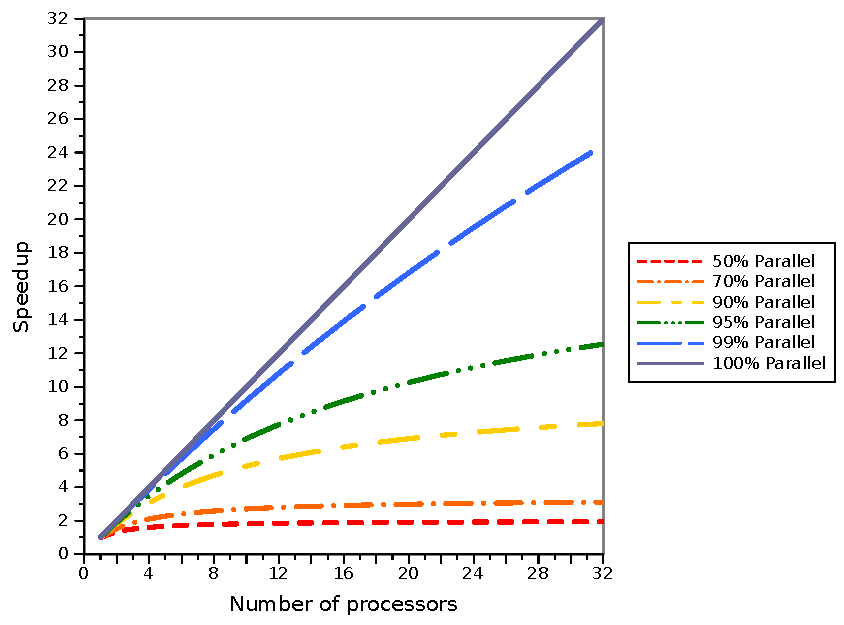
\includegraphics[width=0.5\textwidth]{images/parallel-scaling}
\end{center}


Amdahl's Law tells you how many cores you can hope to leverage in an
execution given a fixed problem size, if you can estimate $P$.

Let us consider an example from~\cite{mte241}: Suppose we have a task that can be executed in 5~s and this task contains a loop that can be parallelized. Let us also say initialization and recombination code in this routine requires 400~ms. So with one processor executing, it would take about 4.6~s to execute the loop. If we split it up and execute on two processors it will take about 2.3~s to execute the loop. Add to that the setup and cleanup time of 0.4~s and we get a total time of 2.7~s. Completing the task in 2.7~s rather than 5~s represents a speedup of about~46\%. Applying the formula, we get the following run times:

\begin{center}
	\begin{tabular}{l|l}
	\textbf{Processors} & \textbf{Run Time (s)} \\ \hline
	1 & 5\\
	2 & 2.7\\
	4 & 1.55\\
	8 & 0.975\\
	16 & 0.6875 \\
	32 & 0.54375 \\
	64 & 0.471875 \\
	128 & 0.4359375\\
	\end{tabular}
\end{center}

\paragraph{Consequences of Amdahl's Law.}
For over 30 years, most performance gains did indeed come from
increasing single-processor performance. The main reason that we're
here today is that, as we saw in the video,
single-processor performance gains have hit the wall.

By the way, note that we didn't talk about the cost of synchronization
between threads here. That can drag the performance down even more.

\paragraph{Amdahl's Assumptions.}
Despite Amdahl's pessimism, we still all have multicore computers today.
Why is that? Amdahl's Law assumes that:
\begin{itemize}
    \item problem size is fixed (read on);
    \item the program, or the underlying implementation, behaves the same on 1 processor as on $N$ processors; and
    \item that we can accurately measure runtimes---i.e. that overheads don't matter.
\end{itemize}

\paragraph{Generalizing Amdahl's Law.} We made a simplification,
which was that programs only have one parallel part and one serial part.
Of course, this is not true. The program may have many parts,
each of which we can tune to a different degree.

Let's generalize Amdahl's Law:

\begin{itemize}
\item  $f_1, f_2, \ldots, f_n$: fraction of time in part $n$
\item  $S_{f_1}, S_{f_n}, \ldots, S_{f_n}$: speedup for part $n$
\end{itemize}

Then,
\[\mbox{\em speedup} = \frac{1}{\frac{f_1}{S_{f_1}} + \frac{f_2}{S_{f_2}} + \ldots +
    \frac{f_n}{S_{f_n}}}.\]

\paragraph{Example.} Consider a program with 4 parts in the following scenario:

\begin{center}
    \begin{tabular}{r|r|r|r}
    \multicolumn{2}{l}{} & \multicolumn{2}{|c}{Speedup} \\
    Part & Fraction of Runtime & Option 1 & Option 2\\
    \hline
    1 & 0.55 & 1  & 2\\
    2 & 0.25 & 5  & 1\\
    3 & 0.15 & 3  & 1\\
    4 & 0.05  & 10 & 1\\
    \end{tabular}
\end{center}

    (Note: these speedups don't have to be speedups from parallelization.)
    
  We can implement either Option 1 or Option 2. 
  Which option is better?

  ``Plug and chug'' the numbers:
\begin{itemize}
\item  {\bf Option 1.}

  \[ \mbox{\em speedup} = \frac{1}{0.55 + \frac{0.25}{5} + \frac{0.15}{3} + \frac{0.05}{5}}
    = 1.53  \]

\item  {\bf Option 2.}

  \[\mbox{\em speedup} = \frac{1}{\frac{0.55}{2} + 0.45} = 1.38 \hspace*{5.5em}\]
\end{itemize}

   \paragraph{Empirically estimating parallel speedup $P$.}
Assuming that you know things that are actually really hard to know, here's a formula for estimating speedup. You don't have to commit it to memory:
  \[P_{\mbox{\scriptsize estimated}} = \frac{\frac{1}{\mbox{\em speedup}}-1}{\frac{1}{N}-1}.\]

It's just an estimation, but you can use it to guess the fraction of parallel code, given $N$ and the speedup. You can then use $P_{\mbox{\scriptsize estimated}}$ to predict speedup for a different number of processors.

\subsection*{A more optimistic point of view}
In 1988, John Gustafson pointed
out\footnote{\url{http://www.scl.ameslab.gov/Publications/Gus/AmdahlsLaw/Amdahls.html}}
that Amdahl's Law only applies to fixed-size problems, but that the
point of computers is to deal with bigger and bigger problems.

In particular, you might vary the input size, or the grid resolution,
number of timesteps, etc. When running the software, then, you might
need to hold the running time constant, not the problem size: you're
willing to wait, say, 10 hours for your task to finish, but not 500
hours. So you can change the question to: how big a problem can you
run in 10 hours?

According to Gustafson, scaling up the problem tends to increase the
amount of work in the parallel part of the code, while leaving the
serial part alone. As long as the algorithm is linear, it is possible
to handle linearly larger problems with a linearly larger number of
processors.

Of course, Gustafson's Law works when there is some ``problem-size''
knob you can crank up.  As a practical example, observe Google, which
deals with huge datasets.

\bibliographystyle{alphaurl}
\bibliography{459}


\end{document}
